\chapter{Methodology}

\section{Agile Methodology}
Agile methodologies, a concept solidified in 2001 with the creation of the Agile Manifesto, is the notion of prioritising the delivery of working software and a focus on individuals, including the customer, the developers, and everyone in-between over comprehensive tools, documentation, and rigid plans that are unable to adapt to incoming change. \cite{AgileAlliance1}

As described by Highsmith et al, agile methodologies embrace inevitable change, as opposed to traditional approaches that seek to 'anticipate the complete set of requirements early and reduce cost by eliminating change'. \cite{947100}

\subsection{Adaptation of Scrum}
With prior experience of using agile methodologies in both industry, and in previous academic work, it was quickly decided upon that Scrum would be a suitable candidate framework to adapt and incorporate aspects of to better appropriate it for solo development, and to use it in conjunction with Feature-Driven Development, which would be the primary methodology used.

Scrum is characterised by three primary roles: a Product Owner, a Scrum Master, and a Developer, all of whom carry out unique roles and carry distinct responsibilities within the organisation or development body. In addition, events, such as but not limited to sprints - a fixed unit of time to denote work nominated from a product 'backlog' is to be completed, with regular face-to-face meetings known as daily scrums (or stand-ups), of which the framework derives its name, used to relay progress information and potential setbacks to other members of the team. \cite{Scrum1} In turn, the terminology and analogies used by Scrum, including the name itself, are borrowed from the game of rugby. As stated by Takeuchi et al, 'as in rugby, the ball gets passed within the team as it moves as a unit up the field.' \cite{Hirotaka1}

The main adaptations made to the framework and incorporated into the custom agile methodology used were the assimilation of all roles into a singular role - incorporating the actual development work expected of a software engineer, the responsibilities of a Scrum Master ensuring that the methodology is followed as pragmatically as possible, and the various aspects and duties carried out by a Product Owner, such as communicating and discussing requirements or changes with the customer. \cite{Drumond1}

Secondly and most notably, changes were made to the traditional system of sprints as measurements of time. They were instead simplified into a straightforward timeframe Gantt chart, with date estimates and guidelines that could be modified where necessary, but nevertheless provided an indication of progress and momentum as the ultimate project deadline draws closer. This Gantt chart is available as Appendix \ref{Gantt Chart}.

\subsection{Adaptation of Feature-Driven Development}
\begin{figure}[h]
    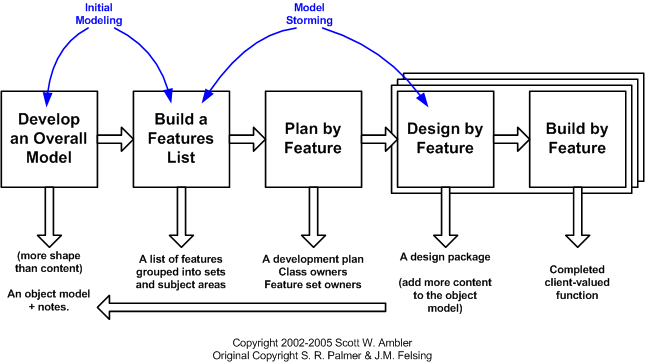
\includegraphics[width=\textwidth]{Figures/fdd}
    \caption{The Feature-Driven Development Lifecycle}
    \label{fig:fdd1}
\end{figure}

With a well-laid out set of initial requirements defined at the start of the project, Feature-Driven Development was determined to be the most appropriate methodology for use with the project alongside the aforementioned adaptations adopted from Scrum. The concept, consisting of the five processes shown in figure \ref{fig:fdd1} was formulated in 1997 by Jeff Luca in order to aid the software development needs of a bank in Singapore. \cite{Arrk1} These processes can be broken down as follows:

\begin{enumerate}
    \item Develop an Overall Model
    \begin{itemize}
        \item The first step is to produce what is, as described by Goyal, a 'high-level walkthrough of the scope of the system and its context.' \cite{Goyal1}
    \end{itemize}
    \item Build a Features List
    \begin{itemize}
        \item The second process is to produce a hierarchical list of features, typically organised by category. \cite{Goyal1}
    \end{itemize}
    \item Plan By Feature
    \begin{itemize}
        \item The third process determines the order in which features are developed, and typically would also involve the distribution of tasks to team members. \cite{Goyal1}
    \end{itemize}
    \item Design by Feature
    \begin{itemize}
        \item According to Karam, the lead programmer selects what features will be developed next, and a domain expert is expected to begin analysing and 'designing a solution to each feature.' \cite{Karam1}
    \end{itemize}
    \item Build by Feature
    \begin{itemize}
        \item Development work on the nominated features begins, and Karam goes on to further explain, that unit tests should also be produced to ensure that the code produced meets the expectations of the lead programmer. \cite{Karam1}
    \end{itemize}
\end{enumerate}

As a result of the usage of this methodology, with the only notable modification being the consolidation of roles into a single person, a detailed design and feature list derived from the functional requirements more adherent to Feature-Driven Development was produced following an analysis and decision on the technologies that would be used, and is explored in detail in Design.

\section{Version Control}
Version control in software engineering began as the adoption of best practices and techniques that were used in neighbouring fields of industrial manufacturing and design, predominantly for the similarly complex drawings and blueprints of advanced components. \cite{Carstensen1} Today, the vast majority of software projects depend on Git - an open source, distributed version control system (DVCS) that was developed by Linus Torvalds originally for use in Linux kernel development, further popularised by online repository hosts such as GitHub. \cite{LinuxFoundation1}

This project makes use of a Git repository in order to track changes and a historical record that can be reverted back to should code regressions or decision changes be made, as well as keeping an online copy uploaded to the GitHub online repository hosting service so that it is additionally protected against accidental deletion or corruption. The use of Git nevertheless complements agile development even as a solo developer, as Robinson elaborates that 'simply being able to see changes and go back to an earlier version can be a huge help.' \cite{Robinson1}

\section{Supporting Technologies}
This section explores some of the computer applications that were used in order to aid the implementation of the explored hybrid methodology.

\subsection{Discord}
\begin{figure}[h]
    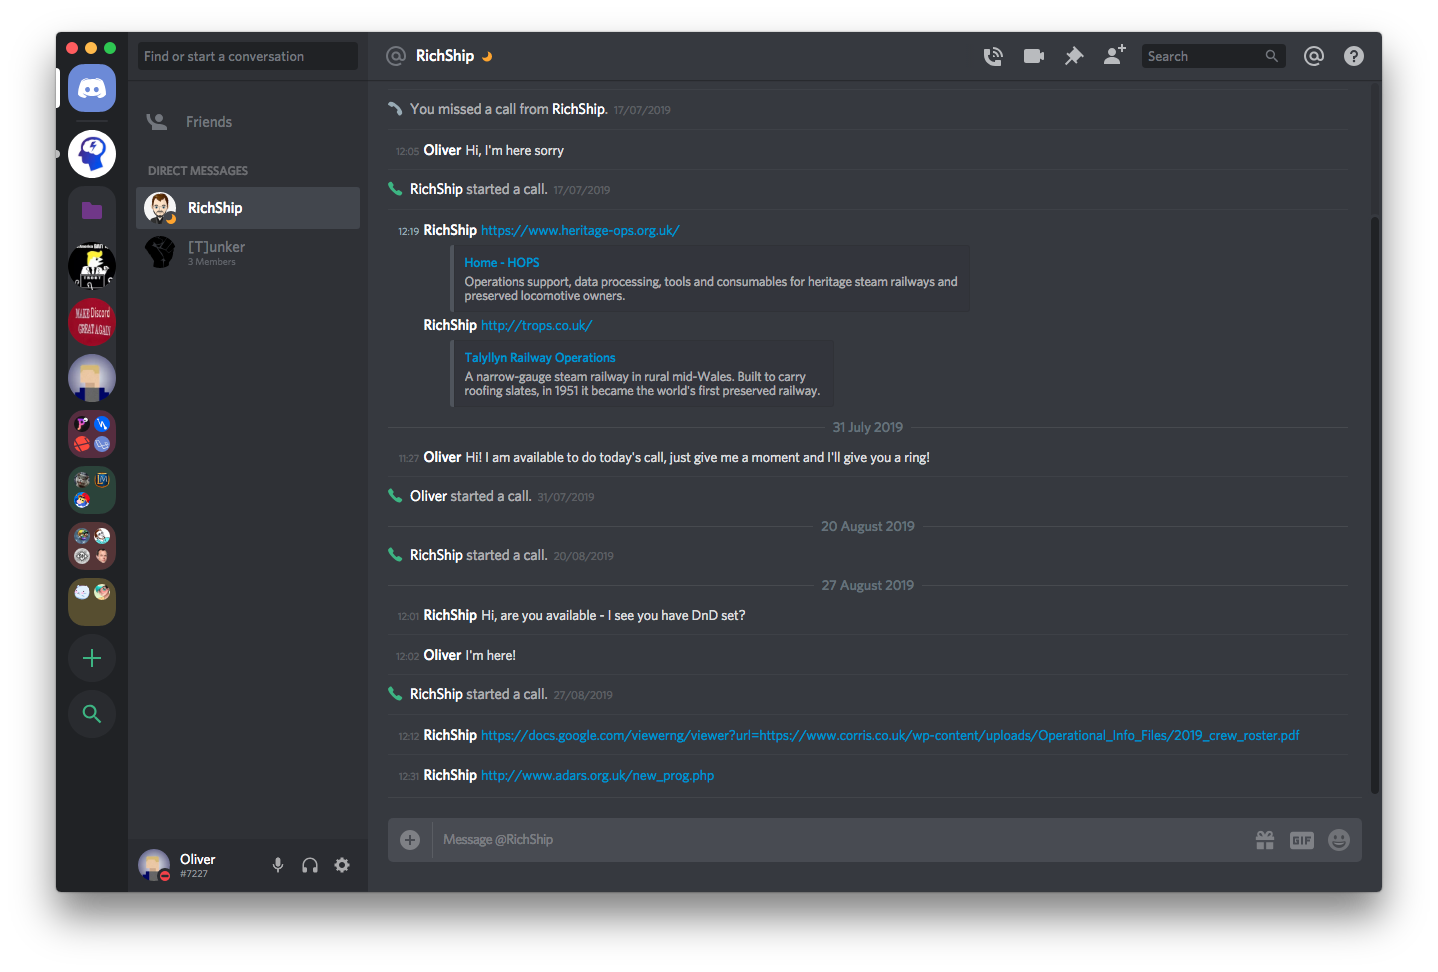
\includegraphics[width=\textwidth]{Figures/discord}
    \caption{A screenshot showing communication history between client and developer, in Discord.}
    \label{fig:discord1}
\end{figure}

Communication, particularly face-to-face communication is an important component of agile methodologies, as described by Inzaurraga as 'making the feedback cycle faster' and 'ensuring development meets the client's expectations'. \cite{Inzaurraga1} The further importance of face-to-face communication is emphasised by Cao et al, who state that such communication 'obviates the need for time-consuming documentation and approval processes' and that it allows 'customers to steer the project in unanticipated directions.' \cite{4420071}

Due to geographical constraints making face-to-face communication difficult, an ideal alternative is audio and video conferencing, which Discord was quickly mutually decided upon to be the facilitatory technology. Discord is a proprietary Voice over IP (VoIP) application available for desktop and for mobile platforms, or usable in a web browser, with functionality including voice and video calling, and importantly, the ability to share a user's desktop view with call participants, a feature known as screen sharing. \cite{Melcon1} Despite the program originally being designed for use by those interested in video games, the application has quickly grown in appeal to other audiences, and competes openly with popular rival messaging and VoIP software, such as Microsoft's Skype. \cite{Giret1}

Weekly voice and video meetings with shared screens were conducted with the client using Discord, as well as facilitating immediate, ad-hoc instant messaging and link sharing whenever necessary, as shown in figure \ref{fig:discord1}.

\subsection{Microsoft Outlook}
\begin{figure}[h]
    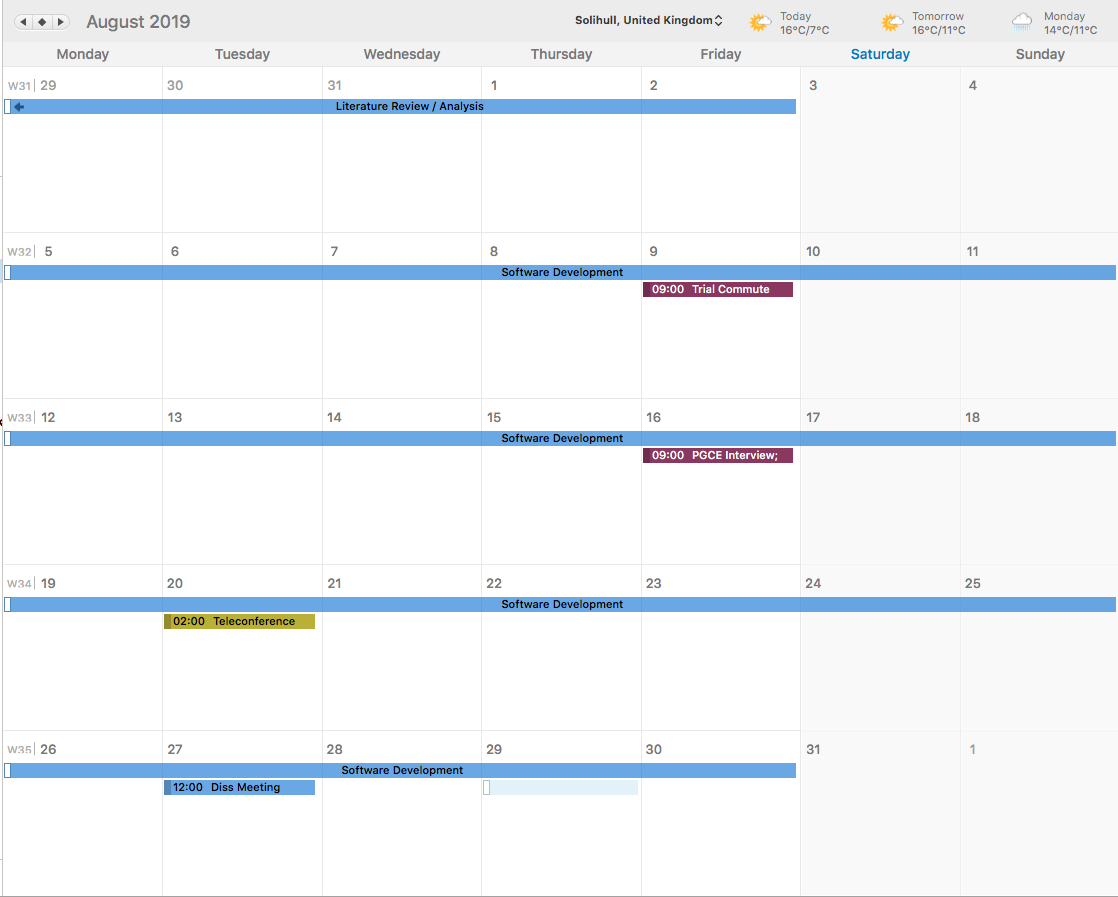
\includegraphics[width=\textwidth]{Figures/outlook}
    \caption{Calendar view in Microsoft Outlook, displaying development time periods.}
    \label{fig:outlook1}
\end{figure}

In order to ensure that development remains disciplined and that the timeframes illustrated in Appendix \ref{Gantt Chart} are maintained as closely as possible, the date durations were added to an appointments calendar within Microsoft Outlook, a popular email, calendar, and newsgroup client developed by Microsoft for Windows and macOS, \cite{Microsoft1} which provided reminders as deadlines approached and as demonstrated by figure \ref{fig:outlook1} were easily viewable at a glance.

While more fitting alternatives for agile software development exist, such as facilities provided by GitHub itself, and also solutions such as Atlassian JIRA, this solution works fine and does not violate the popular KISS (Keep it simple, stupid) principle - a notion that originated in aeronautics, but has since become popular among many branches of engineering, software included. \cite{Branson1}

\subsection{Evernote}
\begin{figure}[h]
    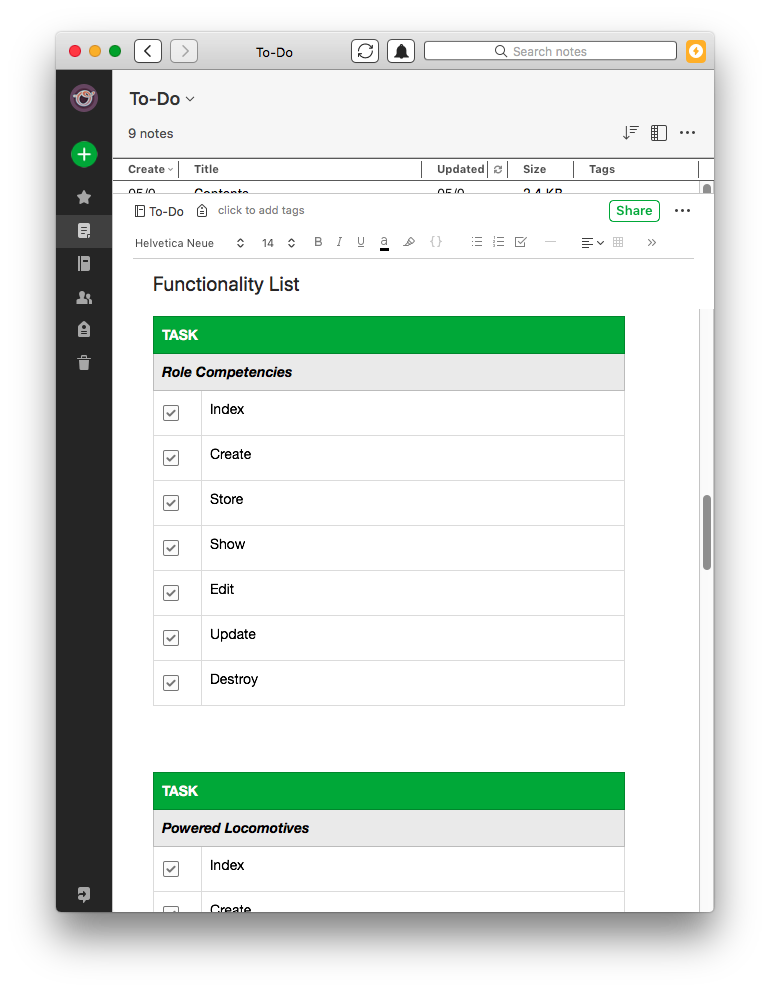
\includegraphics[width=\textwidth]{Figures/evernote}
    \caption{An example of feature checklists displayed in Evernote.}
    \label{fig:evernote1}
\end{figure}

Evernote is a notepad application with a wealth of rich-text formatting features, pre-built templates, and cloud synchronisation support. As it includes ready-to-use templates for to-do lists, complete with clickable checkboxes, it a useful tool for quickly keeping track of functionality that was deemed complete and fully tested. \cite{McCracken1} This proved satisfactory for solo development, although for cooperative undertakings, more specialised tools such as the aforementioned Atlassian JIRA, or the use of a Kanban board would be more optimal.